\documentclass[12pt,preprint,pdftex]{aastex}
\newcounter{address}
\newcommand{\project}[1]{\textsl{#1}}
\newcommand{\units}[1]{\mathrm{#1}}
\renewcommand{\mag}{\units{mag}}
\renewcommand{\arcmin}{\units{arcmin}}
\renewcommand{\arcsec}{\units{arcsec}}
\newcommand{\documentname}{\textsl{Article}}
\newcommand{\sectionname}{Section}
\newcommand{\sectionnames}{\sectionname s}
\newcommand{\rfifty}{r_{50}}
\newcommand{\rninety}{r_{90}}
\newcommand{\hfifty}{h_{50}}
\newcommand{\hninety}{h_{90}}
\newcommand{\conc}{C}
\newcommand{\foreign}[1]{\emph{#1}}
\newcommand{\etal}{\foreign{et\,al.}}
\begin{document}

\title{
       The SDSS Large Galaxy Atlas
      }
\author{
        Ekta Patel\altaffilmark{\ref{CCPP}},
        David Mykytyn\altaffilmark{\ref{CCPP}},
        David W. Hogg\altaffilmark{\ref{CCPP},\ref{MPIA},\ref{email}},
        Dustin Lang\altaffilmark{\ref{CMU}}
       }
\setcounter{address}{1}
\altaffiltext{\theaddress}{\stepcounter{address}\label{CCPP} Center
  for Cosmology and Particle Physics, Department of Physics, New York
  University, 4 Washington Place, New York, NY 10003}
\altaffiltext{\theaddress}{\stepcounter{address}\label{MPIA}
  Max-Planck-Institut f\"ur Astronomie, K\"onigstuhl 17, D-69117
  Heidelberg, Germany}
\altaffiltext{\theaddress}{\stepcounter{address}\label{email} To whom
  correspondence should be addressed: \texttt{david.hogg@nyu.edu}}
\altaffiltext{\theaddress}{\stepcounter{address}\label{CMU} Carnegie
  Mellon University}

\begin{abstract}
We present the \project{Sloan Digital Sky Survey Large Galaxy Atlas},
which contains accurate positions and photometry for galaxies with
half-light diameters greater than $1~\arcmin$. The measurement of
galaxies with large angular sizes is challenging, and has rarely been
done well in automated settings.  Issues include that the galaxies
overlap field boundaries, overlap foreground stars, and show detailed
and confusing internal structure at high signal-to-noise.  We take a
generative modeling or likelihood approach to making measurements of
the galaxies, using very simplified few-parameter morphological models
and with the likelihood modified from a standard chi-squared for
robustness.  We show that we can get precise and reliable (though
possibly biased) measurements of colors and surface brightnesses for
very large galaxies ($>1~\arcmin$ in diameter) in the \project{Sloan
  Digital Sky Survey} imaging data. The parent sample of galaxy
targets was constructed from the Third Reference Catalog of Bright
Galaxies (RC3) and the NASA-Sloan Atlas (NSA). Because the parent
sample is gathered from heterogeneous sources, it is not expected to
be complete, especially at the lowest surface brightnesses.  Our
sample includes measurements of galaxies with radii as large as $\sim
200\,\arcsec$ in radius (such as M101), while
retaining consistency in galactic properties compared to galaxies of
smaller radii.
\end{abstract}
%HOGG: discuss general issue that our photometry is being done the way it is to meet particular goals

\section{Introduction}
The \project{Sloan Digital Sky Survey} (\project{SDSS}) and its
successor projects \project{SDSS-II} and \project{SDSS-III} have had
enormous impact, forming the observational basis for literally
\emph{thousands} of refereed papers.  The success of these surveys can
be attributed to multiple factors, not least the unaccountable
diversity of phenomenology presented to us by our fecund Universe.
One significant factor has been the fact that these surveys have
endeavored to produce and distribute (to the public) reliable,
calibrated, easy-to-use photometric and spectroscopic data.

All that said, the goals of the \project{SDSS} were heavily weighted
towards galaxies and stars with visible brightnesses around 18~mag.
The camera, observing strategy, and data-reduction pipelines were all
optimized for performance at 15 to 22~mag.  Importantly---and to the
chagrin of some investigators (HOGG:CITE SOMETHING)---the \project{SDSS}
photometry of very bright, nearby galaxies has been substantially
biased.  The dominant reason for this is that the \project{SDSS-I}
photometric pipelines employed an ``aggressive'' sky estimation
algorithm that removed much of the light from sources with large
angular footprints, though it has left behind some beautiful images.
A secondary reason is that the ``deblending'' heuristics for
disentangling the light in overlapping galaxies do not deal well with
sources that are hundreds or thousands of times the solid angle of the
core of the point-spread function.

The nearby galaxies are interesting and important!  Because the
\project{SDSS} is supremely well calibrated photometrically, and
because it is a drift-scanning survey, it is particularly well suited
to measuring these objects with large angular extents.  In this
\documentname, we make an attempt to photometer some nearby galaxies
in the \project{SDSS} imaging data and test the precision of those
measurements.

This project has been made possible by two developments.  The first is
that for \project{SDSS-III}, a new global, continuous sky function was
fit to the imaging data, fit to the ``blank'' pixels \citep{blanton11}.  This sky
function does not remove light from large galaxies, or not nearly as
much as previous generations of sky algorithms.  The second is that we
have developed a package \project{The Tractor} (HOGG CITE) for fitting
probabilistic models to astronomical imaging data and the
\project{SDSS} imaging in particular.

In what follows, we fit \project{SDSS} imaging
data on and near large angular-size galaxies using simple (inflexible)
models---mixtures of exponential and de~Vaucouleurs models.  For each
galaxy, we use \project{The Tractor} to
optimize a justifiable scalar objective function that is an
approximation to a likelihood, with modifications to make the fitting
less sensitive (than traditionally) to outliers and morphological
oddities in the galaxies.  The galaxies are typically as large as or
larger than an individual \project{SDSS} frame, but \project{The
  Tractor} doesn't need a co-add or mosaic of the data; it fits all
the individual disjoint science exposures simultaneously.  For most
galaxies we look at, the simple models we are using are \emph{not}
good fits: They can't be, because they don't capture spiral arms, HII
regions, dust lanes, or other morphological non-trivialities.
However, as we will show, they produce precise, robust photometry that
appears to be invariant with galaxy angular size or distance.

There has been much work done fitting big, bright galaxies, sometimes
with very flexible models and sometimes with very rigid ones. In
\cite{simard11}, four different decomposition procedures are used to
make improvements to sky estimations and three different galaxy
fitting models are compared in the g and r bandpasses of Sloan Legacy
Data. The galaxy models include a pure Sersic model, $n_b=4$
bulge$+$disk model, and a model where $n_b$ is a free range between
0.5 and 8 bulge$+$disk model. The most appropriate galaxy model was
chosen using the F-test probability, which estimates reduced chi-squared of
the fit residuals and the number of resolution elements per fit for
each model where $n_{res}=n_{pix,unmasked}/ \pi\theta^2$ and $\theta$
is the r-band seeing at HWHM. To test these methods on a sample of
1.2 million SDSS galaxies, both \verb|SExtractor| and model photometry were used
to deblend and identify object-sky boundaries. The results show that
galaxies with B/T(bulge-to-total-mass) ratios between 0.2 and 0.45
definitely require bulge$+$disk decomposition for best results,
whereas any galaxy with a B/T ratio $>$ 0.75 do not require complex
decomposition.

\cite{lackner} also uses a bulge$+$disk decomposition method for SDSS
galaxies in the redshift range of 0.003 to 0.5 with magnitudes $<$
17.7 in all bands. Five galaxy fitting methods are used by Lackner and
Gunn. They include: deV bulge$+$Exp disk, Exp bulge$+$Exp disk, Sersic
profile, Exp disk profile (n$=$1), deV profile(n$=$4).Two samples were
chosen to test the results, the first sample includes 39 bright
galaxies used to test the degrading of S/N and the second sample
includes 190 galaxies spanning the redshift range of the sample. The
preferred fitting method for each galaxy was chosen by using the
following criteria where bulge$+$disk models are used if the criteria
are true: if the bulge and disk fluxes in the linearly scaled g and i
bandpasses are nonzero, if the bulge scale length is smaller than the
disk scale length, if the bulge flux dominates in the center of the
galaxy, and if the two component fit is significantly better than the
single component fit. Overall, about 29\% were fit with the B$+$D
model, 23\% fit with the single Exp, 13\% fit with the single deV, and
36\% fit with the sersic profile.

In \cite{mcdonald}, bulge$+$disk decompositions are performed on 286
Virgo cluster galaxies. Specifically, the bulge$+$disk decompositions
are used to measure how much light each galaxy contributes. The bulge
model is described by a generalized Sersic function and the disk model
is represented by an exponential function. For spiral galaxies and
irregular galaxies, a combination of the disk and bulge profiles are
used to fit the galaxy. If however, the inclusion of the two profiles
does not improve the fit, the entire measurement is discarded and a
single exponential or sersic profile is implemented. For each galaxy
the u,g,r,i,z, and H surface brightness profiles are extracted and the
bulge$+$disk decompositions are carried out in all 5 Sloan
bandpasses. This collection of data provides a good comparison for
those who want to study structural paramaters and high redshift galaxy
samples.

Multi-gaussian expansion methods have also been used for building
models of galaxies.\cite{emsellem} improves on prior methods which
used centered Gaussians and PSFs containing a single 2D Gaussian by
creating a more general approach using arbitrary PSFs and non-centered
Gaussians. Together, these generalizations also account for
non-centered components of galaxies such as offset bars and disks. The
multi-gaussian method sums PSFs composed of 2D Gaussians that are each
described by the following six free parameters: maximum intensity,
standard deviation, axial ratio, cartesian coordinates of the maximum
intensity(in x and y), and a position angle of the major axis. The
deconvolved and convolved surface brightness are also sums of
Gaussians. For the surface brightness model, a non-linear
least-squares fit program computes a multi-gaussian approximation for
the PSF image where the fixed parameters are the number of Gaussians
and the requested accuracy. This process is flexible in that it
identifies bad regions of the image, allows for binning of the low
intensity regions to avoid consequences of low S/N, and it takes both
linear and non-linear constraints on parameters. By using these
options, this model can be subtracted from the image, leaving an
uncontaminated PSF image. This surface brightness model offers a
robust deconvolution technique, but it depends on some assumptions
which are: the PSF image must be well approximated by a sum of 2D
non-centered Gaussians, the PSF may vary in the field which causes and
accuracy limitation, and the true surface brightness must be well
represented by the sum of non-centered 2D Gaussians. Although perfect
deconvolution is not expected, even partial deconvolution shows that
the deconvolved models improve in resoluton relative to the original
data.

Galaxies show enormous diversity, and no simple model (exponential or
de~Vaucouleurs or mixture of those) is---in any technical sense---a
good fit to the data.  However, simple models are very valuable when
the goal is \emph{consistency} of photometric measurement across size
or distance or data quality.  As data quality or angular resolution
improves, or distance decreases, it becomes easier to fit more and
more complex models.  However, if the goal is consistent model fitting
across populations or data that span different resolutions, rigid
models are preferred.  We provide a lot more philosophical argument
along these lines in \ref{sec:philosophy}; suffice it to say that here
we exploit rigid models to deliver consistent photometry for this
collection of very heterogenous galaxies.

\section{Imaging Data}\label{sec:data}
The imaging data for this project come from the \project{Sloan Digital
  Sky Survey} fully public \project{Data Release 8} \citep{dr8}, which is
the first data release of the \project{SDSS-III} project \citep{sdssiii}.  It
includes fully recalibrated imaging \citep{padmanabhan} from the
combined imaging projects of \project{SDSS} \citep{york}  and
\project{SDSS-II} \citep{sdssii}.

The fitting code (\project{The Tractor}, described briefly below, and
more completely in Lang \etal, forthcoming) locates \project{SDSS}
imaging fields that overlap a large circular footprint centered on the
pre-fitting (input) galaxy center.  It downloads (on the fly)
\project{DR8} imaging data files corresponding to those fields from
the \project{SDSS-III} \project{Data Archive Server} (HOGG:CITE?).  The
downloaded data files are the photometrically calibrated,
background-subtracted ``frames'' files.

For every pixel of the imaging, we construct an approximate ``inverse
variance'' value, which is the reciprocal of the variance expected
given the Poisson photon, Poisson dark-current, and Gaussian
read-noise error models.  In detail, we use the equations recommended
by the \project{SDSS-III}
Collaboration.\footnote{\url{http://data.sdss3.org/datamodel/files/BOSS\_PHOTOOBJ/frames/RERUN/RUN/CAMCOL/frame.html}}
We set the inverse variance to zero for any pixels that lie in regions
that were interpolated, saturated, or affected by cosmic rays or ghost
images.

For the PSF model, we use the SDSS double-Gaussian model stored in the
``psField'' file.  DSTN: What do we get as parameters for that
double-Gaussian model?  I think it is less than 1 + 4 + 6 parameters
that a K=2 D=2 MoG would have, right?

\section{Input Catalogs}
We aim to create a catalog with a similar structure to the
\textit{GALEX} Ultraviolet Atlas of Nearby Galaxies. It provides
photometry, surface brightness and color profiles for 1034 nearby
galaxies with a diameter larger than $1~\arcmin$ and a surface
brightness in the b-band, $u_B$=25 mag arcsec$^{-2}$ . The galaxies
chosen for this data set come from the \textit{GALEX} Nearby Galaxies
Survey and other equivalent\textit{GALEX} initiatives that viewed the
same fields of the sky in the far-ultra violet(FUV) and near-ultra
violet(NUV) bands. All galaxies with a diameter larger than
$1~\arcmin$ from RC3 were also added to the sample. A total of 81 out
of 1136 galaxies were not included in the \emph{GALEX} UV Atlas of
Nearby Galaxies because they were in regions of very high background,
high Galactic extinction, extremely low UV surface brightness, or
simply had images that were not of sufficient quality for
analysis. The surface brightness was measured using the central
position, ellipticity, and position angle of the $D_{25}$ ellipse. It is
computed to within the annuli of ellipse's central angle increasing
out by $6~\arcsec$ from the major-axis until it reaches at least 1.5
times $D_{25}$. Point sources in the images with colors redder than
FUV-NUV=1 were automatically masked and visually checked. After the
\verb|SExtractor|-detected\citep{sextractor} sources were masked within a 5x5 pixel
range of each source, the mean of the sky was used as the estimate of
the background. Galactic color excess is taken from
\cite{schlegel98} and used with the extinction law from
\cite{cardelli}. The surface brightness profiles were then used to
compute asymptotic magnitudes, colors, luminosities and
concentrations. Magnitudes, effective radii, and colors were found by
extrapolating growth curves to infinity and performing error-weighted
linear fits. The morphology of the UV surface brightness profiles were
determined visually using a two-letter naming scheme, the first
describing the outer profile and the second describing the inner
profile \citep{gdp06}.

The initial input catalog of galaxies for our project was formed out of the union of the Third
Reference Catalog of Bright Galaxies (RC3), the NASA-Sloan Atlas
(NSA), and the 2MASS Large Galaxy Atlas (LGA). Objects with an angular
diameter greater than or equal to 1 arcminute were selected. 

The RC3 catalog, which contributes the most galaxies to our data set,
gives methods of measurements in Volume I of the catalog. Positions
for the galaxies contained in RC3 were measured using the SAO Star
Catalog and the FK4 coordinate system, but are listed by the 2000.0
equinox positions. A large number of positions were also taken from
the CGCG, UGC, and MCG catalogs. $D_{25}$ was measured at the 25.0
B-m/ss level in units of 0.1 arcminutes. The isophotal diameters are
largely taken from three sources including derivations from de
Vaucouleur's photoelectrically calibrated photographic and CCD
photometry, interpolation of R. Buta's\citep{buta} photoelectric
growth curves, and from the photoelectric calibration of surface
photometry by Lauberts and Valentijn\citep{lauberts} from which the
largest contributions are made to RC3's $D_{25}$ values. Galactic
extinction was measured using the Burstein \& Heiles\citep{bh} method,
which involves a combination of local galacatic HI column densities
and faint galaxy counts. Internal extinction is measured
by \begin{equation} A_i= \alpha(T)log(R_{25}) \end{equation} where
$\alpha(T)$ is a coefficient dependent on morphological type and
$R_{25}$ is the axis ratio. Various magnitudes were measured and
included in the RC3 catalog. The total photoelectric magnitudes,
$B_T$, were found using two methods which are the extrapolation of
photoelectric aperture photometry using standard curves and the
extrapolation of the calibrated surface photometry. Two different
surface brightnesses are included. One measures the mean effective
surface brightness with the effective aperture, $A_e$. The other
method measures the mean surface brightness within the $D_{25}$
ellipse, using the the axis ratio,$R_{25}$\citep{rc3}.  In RC3, the
search for galaxies to include our sample was based on the measured
apparent major isophotal diameter at the surface brightness
level$\mu_{B}=25.0$ mag in 1 arcsec$^2$ arcsecond of $D_{25}$ $>$ 1
arcminute.

The Nasa-Sloan Atlas(NSA)\footnote{\url{www.nsatlas.org}}
rephotometered all redshifts for galaxies within the SDSS Data Release
8. It takes the images from the \textit{ugriz} bands of SDSS and the
NUV and FUV bands from \textit{GALEX}. The methods used in the NSA is
an improvement to those used by SDSS. It begins with an estimation of
the sky from a processed SDSS image and creates masks for all bright
sources in and around the image. A spline is fit to the unmasked data
with constraints that make the process run even for images where heavy
masking is needed \citep{blanton11}. In the NSA, we checked for any
objects of significant size that were not also in RC3. This includes
objects with a 50\% light radius of the SERSIC fit greater than 30
arcseconds. The objects were then examined by eye to determine which
ones were actually large galaxies and which were errors in the
NSA. Examples of errors include stars causing saturation, interstellar
medium, and nebulae. Some interesting galaxies that were not contained
in RC3 were found and measured and have been included in the SDSS
Large Galaxt Atlas(hereafter, SDSS LGA). A subset of these images
contained two galaxies, which we fit individually.

EP:how does NSA improve the SDSS background?...
 
The 2MASS Large Galaxy Atlas(LGA) provides near-infrared photometry
for large galaxies in an attempt to connect the gap between optical
wavelengths and longer wavelengths. We have checked for galaxies in
the LGA that were not included in RC3 and had an isophotal fiduciary
radius in the K-band of $1\arcmin$(or is this 30 arcsec??) or
more. The only objects found were either missing in the SDSS imaging
data or were globular clusters.  \citep{jarrett03}.

\section{Method} \label{sec:method}
\subsection{Galaxy photometry is impossible}\label{sec:philosophy}

There is a deep sense in which obtaining precise and accurate galaxy
photometry is fundamentally impossible.  The reasons are multiple, but
the dominant reasons are, first, that the angular outskirts of
galaxies can contain significant luminosity but at incredibly low
surface brightness and unknown morphology, and secondly, that the
imaging point-spread function (PSF) can also have large-angle
contributions that are unknown.  The latter problem affects stellar
photometry also, but so long as the PSF is constant, precise and
accurate stellar photometry \emph{is} possible.  The difference
between galaxies and stars is that all point-like stars will
illuminate the PSF (correlate with it) identically.  Stellar
photometry does not rely on getting all this right so long as it deals
with it \emph{consistently} across stars.  Not so for galaxies, each
of which might have very different correlations with the PSF at large
angles.  There is no way to produce consistent photometry without
knowing things about every galaxy and every PSF that are---almost in
principle---unknowable.

These fundamental issues and also many pragmatic issues of noisy,
badly calibrated, and crowded imaging have forced astronomers to
consider many different methods for measuring galaxy fluxes.  Each has
flaws.  Here we give a highly biased and very brief review.
\begin{itemize}
\item Given digital imaging of a patch of sky that includes a galaxy,
  the simplest way to measure the flux of that galaxy is
  \emph{aperture photometry}.  This is the measurement of the total
  light (the integral of the intensity, found by summing pixel values)
  in the image above the sky (foreground and background) intensity
  within a fixed circular angular aperture, centered on the galaxy.
  This kind of photometry obtains different fractions of the galaxy
  light in galaxies that have different proper sizes or which lie at
  different radial (angular-diameter) distances; in this sense it
  does not produce photometry that is distance-independent.  It has
  many other problems as well, some of which will come up later in
  this list.
\item Aperture photometry can in principle be improved by scaling the
  radius of the aperture with the inverse radial (angular-diameter)
  distance to the galaxy.  This helps in making the photometry
  distance-independent, but it requires prior knowledge of the galaxy
  distances.  It also does not perfectly compensate for distance
  because galaxies at different distances are subject to the same (in
  angular size) PSF illuminate even though the properly scaled apertures
  differ.  This change also does not account for galaxies with
  different proper sizes.
\item Aperture photometry can be made adaptive, adapting the aperture
  to the observed angular size of each galaxy.  This requires image
  analysis---galaxy size measurement---prior to the photometry.  In
  one extreme version, \emph{Isophotal photometry}, the photometric
  aperture is made the (usually very non-trivial) precise \emph{shape}
  of a particular intensity contour in the galaxy image.  Isophotal
  photometry is close to distance-independent for low-redshift
  galaxies; at high redshift relativistic intensity dimming
  ($[1+z]^{-4}$) breaks that symmetry.  Also, isophotal photometry
  will in general get very different fractions of the galaxy light
  from high and low surface-brightness galaxies.  It also remains at
  least slightly dependent on the PSF for the same reasons as the
  previous methods.
\item \emph{Petrosian photometry} \citep{petrosian} adapts the angular radius of
  the photometry aperture using a statistic of the galaxy profile that
  is insensitive to total surface brightness.  It works by identifying
  a radius at which the (azimuthally averaged) intensity is a fixed
  fraction of the mean within that radius.  Again, this method is at
  least slightly dependent on distance because of the PSF.
\item The most adaptive methods in common use---not the most adaptive
  \emph{possible}---involve measuring the galaxy's \emph{radial
    profile} by averaging the intensity above the sky intensity in
  narrow circular (or sometimes elliptical) annuli centered on the
  galaxy, and then summing the annular contributions to the flux, and
  maybe also extrapolating at large radius.  These methods are usually
  designed to attempt to get ``all the light''.  They do not overcome
  the fundamental problem of large-radius galaxy and PSF morphology.
\item One problem in common to all the above approaches is that they
  involve ``adding up'' the flux in pixels.  This arithmetic operation
  creates what is classically called a ``statistic'' of the data; it
  will not be the minimum-variance estimator of anything.  That is, if
  information preservation or precision is of high value, none of the
  above methods are palatable.  Information-preserving inference
  requires fitting probabilistic models, with a likelihood funtion at
  least and maybe also informative priors.  In the enormous
  \project{Sloan Digital Sky Survey}, despite the fact that aperture
  and Petrosian magnitudes were measured and published, it was the
  magnitudes based on \emph{model fitting} that got the most use: They
  produced more precise colors.  It is also the case that model
  fitting is the first method in this list that has a shot at
  producing truly distance-independent measurements because a
  component of the model fit is the PSF.  Inasmuch as the galaxy and
  PSF models are appropriate and correct, model fitting is in some
  sense probably the best way to measure galaxy photometry.  Of course
  it does not overcome the fundamental problems of galaxy photometry
  with which this \documentname\ opens: We do not understand galaxy
  profiles or the PSF at large angular radii, and though there can be
  significant light out there, it is hard to find in the data.
  Furthermore, in the standard methodologies of model fitting,
  extremely simple galaxy models are used, such as elliptical
  exponentials and de~Vaucouleurs profiles \citep{dev}.  These smooth
  models are not at all a good description of two-dimensional images
  of most real galaxies at \emph{any} angular radius (think: spiral
  arms, bars, rings, HII regions, dust lanes, and so on).
\item An almost unexplored territory for galaxy photometry is to
  consider extremely flexible galaxy models, models so flexible that
  they can capture all of the details.  This would require a
  significant technical investment and a lot of computer time, but it
  might pay off.  It ought to give the best measurements in the end;
  it is the ultimate in ``letting the data decide''.  However, even
  this flexible approach will not overcome the fundamental problems; in
  some sense the true, total photometry of a galaxy is \emph{not an
    observable}.
\end{itemize}
All the problems with these different photometric measurement
techniques flow into the subsequent or simultaneous measurements made
of other quantities of interest, like sizes, concentrations, surface
brightnesses, and so-on, because these measurements are (or involve)
transformations of photometric measurements.  The best choice among
techniques will depend on the uses to which the measurements are going
to be put; in some cases precision is paramount, in others consistency
across distance, in others robustness to varying PSF, in others
consistency across morphological types.

In this project, our goal is to obtain consistent multi-band
photometry for a large set of galaxies at a wide range of distances,
with a large range of morphologies, surface-brightnesses, and angular
sizes relative to the PSF.  Importantly, we want to do the very
(angularly) large galaxies in the same way as we do the (angularly)
compact.  Consistency is more important than accuracy, in the sense
that we would like to get numbers that---if they must be wrong---are
wrong \emph{in the same way} for the \emph{same galaxy} observed at
different distances or through different atmospheric PSFs.  We also
want precision---we want to avoid introducing unnecessary scatter or
noise by our choice of procedure.

These considerations argue \emph{for} probabilistic modeling and
\emph{against} using very flexible models.  We are making a catalog of
photometry, not delivering posterior PDFs; our photometry will
therefore contain \emph{estimators} for flux, color, size, and so-on.
Minimum variance estimators are maximum-likelihood estimators, so we
will only consider approaches in which we (under assumptions)
construct an approximate likelihood function and optimize it.  As we
note above, the requirement that our photometry be distance and
PSF-independent also argues for modeling approaches.  The reason we
prefer inflexible models to flexible models is that at the optimum in
the likelihood, a large angular-size galaxy will exercise much more
model freedom than a small angular-size galaxy: In the large galaxy,
many more features and details are visible under finite PSF.  Again,
distance and PSF consistency requires that we restrict model freedom
identically or as identically as possible for all galaxies we measure.
This argues for overly simplistic models; the models we will use below
do \emph{not} capture the full two-dimensional structure of the
galaxies being measured, but (as we will show), they do provide
robust, high signal-to-noise, consistent measurements.

In addition to the photometric issues discussed above, there are a
large number of separate pragmatic issues when we consider the problem
of performing galaxy photometry automatically and consistently in a
large and heterogeneous data set.  When galaxies are angularly large,
as they will be here, they often overlap stars.  Bright stars make it
hard to precisely measure the fainter galaxy.  Faint stars are
challenging to deblend from the galaxy reliably.

In addition to overlapping stars, galaxies frequently overlap other
galaxies, both because galaxies are spatially clustered and because
some ``galaxies'' are really pairs of galaxies merging.  Overlapping
galaxies must be ``deblended'', which is a source of consternation in
many imaging surveys.  The consternaton arises both because proper
deblending is an ill-posed problem and because it is very
distance-dependent.  The problem is ill-posed because there is no
definition of the boundary between two galaxies and one; even if there
were, we wouldn't know how to separate the observed intensity into the
two components.  Clever data-driven heuristic proposals and methods
exist (\cite{lupton}, \cite{sextractor}) but nothing is reliable for
angularly large galaxies, where enormous non-smooth detail is visible
for a large range of Hubble types.  Deblending is distance-dependent,
because a galaxy observed nearby is much larger than the PSF; all of
the spiral structure and HII regions are well resolved.  A distant
galaxy is a smooth blob under the PSF.  The deblending simply cannot be
the same if it is based on flexible heuristics.  This is another place
where fitting inflexible models will help us: Although the inflexible
models are never good fits, they provide objective methods for
simultaneously measuring two overlapping galaxies.

\subsection{Measuring Galaxies with \emph{The Tractor}} 

HOGG/DSTN:first a few words about \project{The Tractor}

Models: Write about the types of models used?? Different galaxies
types etc?  

The Tractor functions first by building a model, using
initial parameter data that is supplied. Next, it takes the derivative
of each parameter and performs a weighted least-squares fit to find a
parameter update that will minimize $\chi^2$.  Since this is a
linearization of a non-linear problem, we perform a line search along
the update direction, taking steps of increasing size starting from
$1/1024$ and increasing by factors of $2$ up to a factor of $2$ of the
linear direction; we halt the line-search when the $\chi^2$ stops
decreasing.  Finally, the parameters are updated in that direction. The
tractor is capable of freezing certain parameters, so that they are
excluded from the optimization.The iteratively-reweighted least
squares process is used to update the inverse variances after each
iteration of optimization. The math is:

\begin{eqnarray}
\chi^2 &\equiv& \sum_n \chi_n^2
\\
\chi_n^2 &\equiv& \frac{[d_n - m_n]^2}{\sigma_n^2}
\\
\frac{1}{\sigma_n^2} &\leftarrow& \frac{1}{\sigma_n^2}\,\frac{Q^2}{Q^2+\chi_n^2}
\quad ,
\end{eqnarray}
where $Q$ is the number of ``sigma'' at which the residual saturates. $Q$ for these fittings was chosen to be 5. HOGG/DM: Find out why...

In order to deal with the problems of stars that overlap with the
galaxy which we are interested in, we decided to mask them out. The
stars were found using the data in the Tycho-2 star catalog \citep{tycho2}.
The stars were masked out to a
radius of
\begin{equation}
\theta_{\mathrm{exclude}} = \max(25, 25\,2^{[11\,\mag-V]})
\end{equation}
where $V$ is the visual magnitude given by Tycho-2.
(DSTN:I'm not sure why these values, I got them from Dustin, says DM) The mask was applied by setting the chi values of the masked out pixels to zero.

When given an RA, a Dec, and a radius, \emph{The Tractor} searches the SDSS imaging
data for fields which overlap anywhere in that space. It downloads all
those fields, in all bands, as fits files, and then imports them into
the program as arrays. The initial inverse variances are also
downloaded from SDSS.  Saturated pixels from the SDSS images were
masked and then a binary dilation with three iterations is
applied.

For the purpose of measuring and optimizing on a single galaxy at a
time, all other objects were removed from within a circle centered on
the galaxy center which extended out to its radius given by the source
catalog for that galaxy. This method was used rather than working within the
SDSS catalog data itself because SDSS frequently splits up large galaxies into
numerous frames. As initialization parameters, each galaxy was
given magnitudes of 15 in every band.

We start the fitting with an exponential galaxy and then optimize only
that galaxy six times. Following that, a composite galaxy is
initialized which has both exponential and deVaucouleur
components. These components are free to vary separately in order to
best fit the data. The new composite galaxy is also optimized six
times by itself.

In order to measure the half-light radius $\rfifty$, the 90 \% light
radius $\rninety$ and the concentration parameter $\conc\equiv
\rninety/\rfifty$, we took the model of the galaxy that had been
optimized and placed it in an empty frame within the tractor.  Over a
series of increasing intervals of radii we summed up the total flux
within the circles and then interpolated to find $\rfifty$ and
$\rninety$.  We used sixty-four radii equally spaced in pixel
logarithms from zero to half the height of the image. Exceptional
cases were flagged for later review if $\rfifty$ was not between the
deVaucouleur and exponential radii for that galaxy, and concentration
was flagged as incorrect if $\frac{1}{\conc}$ was not between .29 and
.46.  HOGG: Add citation to paper for these numbers. Over the same
series of concentric, increasing radii, we also measured the contained
flux by summing sixty-four equally spaced rectangles. The rectangles
are oriented diagonally and perpendicular to the length of each
galaxy. To find the proper orientation angle for the increasing
rectangles, we calculated the principal unit eigenvectors using a
variance tensor of the image retrieved from \emph{The Tractor}. Using
the eigenvectors and the individul pixel positions relative to the
center of each galaxy, we calculate *rdotv* to use as a checkpoint to
see if at each radii there is some flux contained within the
rectangle. Using the same interpolation scheme that was used for
$\rfifty$ and $\rninety$, we interpolate to find $\hfifty$ and $\hninety$ in
all bands. As expected, the rectangular integrals of flux increased
much faster than the circular integrals, but they both eventually
converge to the same value after some time. The rectangular method
proves to be especially useful for galaxies that are not circular.

An example of a completed measurement is given for NGC 4605, which has
6 fields, each of which has images in all 5 bandpasses that combined
to make our image. These six are shown separately in Figure
\ref{fig:4605data}. The SDSS data from these fields are shown for the
i-band only. Figure \ref{fig:4605model} shows our completed model for
this galaxy. Figure \ref{fig:4605diff} is the difference between the
data and the model. Finally, Figure \ref{fig:4605chi} shows our chi
values for the galaxy. Figure \ref{fig:colorsdata} shows the data for
each band individually, and Figures \ref{fig:colorsmodel},
\ref{fig:colorsdiff}, \ref{fig:colorschi} shows the results for the
model, the difference between the model and the data, and the chi
values respectively.

\section{Catalog}
\subsection{Post-processing}
With results for each composite galaxy measured by \emph{The Tractor}, we
first applied extinction corrections as given by Schlegel et al. 1998
using the \verb|astropysics|
package.\footnote{\url{packages.python.org/Astropysics}} The
\verb|get_sfd_dust| function in the \verb|obstools| class of the
\verb|astropysics| package allows us to retrieve the reddening value
E(B-V) from the SFD dust maps by converting the RA and Dec for the
composite galaxy to galactic coordinates. The reddening values are
then multiplied by the appropriate coefficients A(V)/E(B-V) per Sloan
bandpass to obtain the total extinction to be subtracted from the
individual magnitudes of each bandpass. The coefficients are the
following: $u=5.155,\;g=3.793,\; r=2.751,\; i=2.086,\; z=1.479$. Both
the total magnitudes for the composite galaxy and the extinction
values for all bands per galaxy are presented in our table. With the
corrected magnitudes, we computed surface brightness in the i-band
with \begin{equation}
  \mu_{50,i}=m_i+2.5log(\pi{r_{50}}^2) \end{equation} where $m_i$ is
the corrected magnitude in the i-band and $r_{50,i}$ is the half-light
radius in the i-band.

\subsection{The Table}
The table of data contains the composite galaxy RA, Dec, and name
given by each galaxy's source catalog. The
data from the composite galaxies also includes the magnitudes,
half-light radii,90 \% light radii, concentrations, axis ratios, and
position angles. See Table 1. 

EP:insert exceptions table and snippet of our final atlas

HOGG: What else, if anything, goes here(EP)?

\subsection{Hand-Vetting}\label{sec:handvetting}
We have made various visual checks for our sample of galaxies, which
have led to a number of manual reruns for improved measurements. In
some cases, the second result provided more valuable measurements,
while in others, the rerun did not seem to improve the original
measurements. For a full list of our comments from visual inspections,
see Table 2. One of the first interesting sets of measured galaxies
that we chose to inspect was the set of all objects tha came from the
NSA and contained a radius larger than 30 $\arcsec$. In many cases,
the galaxies were being obstructed by large stars in the same field as
the galaxy, causing saturation of the image and improper measurement
of the galaxy overall. Other galaxies, however, such as NSA ID 148151
have proven to result in a good fit of the galaxy. Other objects in
this set were simply groups of galaxies, each too small individually
to fulfill the size criteria for our catalog. Lastly, there were some
irregular galaxies with very low surface brightnesses that we have
still managed to measure well such as NSA ID 144510, NSA ID 142450,
and NSA ID 175551. See Figure \ref{fig:outliers}.

After initial measurements of all galaxies in our input sample were
completed, optical images were created for the preliminary atlas
objects using the g,r,and i band photometry. These were sorted by
increasing half-light i-band radius. At this stage, the images and the
consequent flipbooks of measurements were observed for galaxies which
seemed to be flawed in one of the following ways: groups or pairs of
galaxies that should be fit separately, galaxies that were off
center, fields of the sky that appeared to contain no galaxy, or
galaxies with bright stars nearby or overlapping with the image of a
galaxy.

Another set of galaxies that was observed individually, by eye were
those which had an infinite i-band flux after initial fits
were runs. Many of these images had bad sky levels in the i-band due
to groups of galaxies or stars in the vicinity that contributed excess
light to the fit. For some galaxies, the fit did not initialize when
galaxies were not in the center of their fields. For such galaxies, we
reran our fits giving a new intial position from the NASA/IPAC
Extragalactic Database(NED). In most cases, a new
initialization improved the measurement enough to discard the original
fit. Another cause of infinite flux is due to large bright stars in
the background and/or foreground of the galaxies that saturate the
pixels of the galaxy images.

Galaxies that were initially outliers on Figure \ref{fig:outliers}
were investigated as well. In the case where two galaxies were in the
same field, we initialized fits for each individual galaxy. For
merging galaxies, most pairs led to good fits for each galaxy
individually despite the lack of explicit boundaries between the
merging galaxies. NGC 3395 and NGC 3396 are an example of a merging
pair of galaxies that were measured well. See Figure
\ref{fig:gooddouble}. Pairs of galaxies that are not merging, however,
were not as succesful overall. For some pairs, the individual
measurement of one galaxy overtook the fit of the second galaxy,
causing innacurate measurements. An example of a bad fit of a pair of
galaxies is NGC 4649 and NGC 4647. See Figure \ref{fig:baddouble}. For
pairs that did not run as two separate succesful galaxies, we only
include the galaxy that has a better fit. The rest of the outliers in
this set of galaxies were those whose measurements did not initialize
at the location of the galaxy due to the galaxy being off-center in
its field. For these galaxies, new position parameters were given
using NED. A majority of these galaxies showed significant
improvements in their new measurements. In all cases where a galaxy
was an outlier, the new measurement was accepted as good and the
original measurement was discarded unless otherwise noted in Table 2.

Two pairs of galaxies that were rerun as individual galaxies
included companion galaxies that were not included in either
NSA or in RC3. The companions are NED 01, found next to NSA ID
86994 and PGC 1563523, which is found with NGC 52. The companions have
not been included in our table.

The last method used for visualization of our measurements was a
sorting of the galaxies by g-i color into quantiles. A color cut was
made at the 50th percentile of the data and again at the 25th and 75th
percentiles. Each of these quartiles were further split into four more
quartiles each by half-light surface brightness in the i-band. See
Figure \ref{fig:quartiles}. We now have a data set that is divided
into 16 subsets by color and surface brightness. They were labeled
such that the bluest and highest surface brightness galaxies are
flagged with a 0 and the reddest and lowest surface brightness
galaxies are flagged with a 15. See Figure
\ref{fig:quartilediagram}. Again, images using the SDSS g,r, and i
band photometry were created sseparetly for each of the 6 subsets of
data, this time ordered by decreasing 90\% light radius. With these
images, we made comments on galaxies that did not fit the size order
criteria and observed the details of their measurements. In many cases
for galaxies that appeared to be smaller than their measured radius,
the fits were extending too far away from the galactic nucelus,
resulting in extra light collection from the sky value. In some other
cases, nearby stars were being over-masked and consequently masking
pieces of the galaxy in that frame, leading to invalid
measurements. EP/HOGG:What are we doing with those?

\subsection{Exceptions and issues}\label{sec:results}
For the largest of galaxies, SDSS provided many fields where each
field contained images in each of the \textit{ugriz}. Many galaxies in
the Messier catalog, such as M81 had too large of a radius in RC3 to
run successfully through \emph{The Tractor}, so scaling factors were
introduced in the pixel data. The scaling factors are dependent on the
number of fields per galaxy. For those galaxies which had between 10
and 20 fields, the pixels in the fields were scaled down by a factor
of 2. Galaxies with 20 to 40 fields each were scaled down by a factor
of 4. Galaxies with 40 to 80 fields were scaled down by a factor of 8
and those with more than 80 fields could not be run through the
\textit{Tractor} successfully. The binning of the pixels in these fields
did, however, provide sufficient accuracy to within a few percent for
the colors in comparison to colors resulting from no binning.
 M51 and the Mice Galaxies are examples of galaxies for which the
 secondary measurements seemed to be within a few percent error of the
 dense region in Figure \ref{fig:atlasconsistency}.

Some galaxies that were problematic for reasons other than pair of
galaxies, bright stars and off-center images were the edge-on
galaxies.The flexible model used by \emph{The Tractor}, which can
successfully fit galaxies with vastly different morphologies does fail
for the galaxies that are not fully or partially face-on. Figure
\ref{fig:edgeon} shows an example of NGC 5907, an edge-on galaxy that
we cannot measure well.
 
UGC 5613 is another galaxy that does not react well to the methods of
\emph{The Tractor} because it is actually composed of two galaxies
that are in the late stages of merging. Some tidal tails can be seen
in the SDSS phtometry, leading to a bad fit. See Figure
\ref{fig:badsingle}.

All data that was flagged for review after an initial failed fit was
reviewed by examination of the full flipbook for that galaxy.

\section{Discussion}\label{sec:discussion}
We successfully measure consistent colors properties for galaxies of
all sizes, showing that the \emph{The Tractor} is indeed a good tool
to measure galaxies at different distances and of different
morphological types. The color properties have a tight correlation and
improve on those measured by the NSA, shown in Figure
\ref{fig:nsacolors}. It is also clear between Figure
\ref{fig:atlasconsistency} and Figure \ref{fig:nsacolors} that we
provide good measurements across galaxies with varying radii.

The Owl Nebula was included in the list of objects that are not in
RC3, but have been included in the NSA. Though we are not
particularly interested in nebulae, the fit for the Owl Nebula is
succesful. 

HOGG: Why are we getting bad concentration values?\\
HOGG: discuss general issue that our photometry is being done the way it is to meet certain particular goals\\
HOGG: What do we want to say about triangle plot? How do we cite it?\\

\acknowledgements It is a pleasure to thank Michael Blanton(NYU), Dan
Foreman-Mackey(NYU), Douglas Finkbeiner(Harvard), Thomas
Robitaille(MPIA), Jim Gunn (Princeton),
Robert Lupton (Princeton), David Spergel (Princeton) Benjamin
Weaver(NYU), and Stephane Courteau(Queen's College) for valuable
discussions. Funding for the SDSS Large Galaxy Atlas has been provided
by New York University's College of Arts and Science Dean's
Undergraduate Research Fund.This work was supported in part by The
Princeton University Press,NASA (grant NNX12AI50G) and the NSF (grant
IIS-1124794).This research has made use of the NASA/IPAC Extragalactic
Database (NED) which is operated by the Jet Propulsion Laboratory,
California Institute of Technology, under contract with the National
Aeronautics and Space Administration.

HOGG: Insert relevant SDSS boilerplate here...

The code for the methods used to make the measurements in this catalog
can be found at: www.github/davidwhogg/SloanAtlas

\begin{thebibliography}{70}
\bibitem[Abazajian \etal(2009)]{sdssii} 
%The Seventh Data Release of the Sloan Digital Sky Survey
Abazajian, ~K.\etal, 2009. \apjs~182, 543

\bibitem[Aihara \etal(2011)]{dr8}
Aihara, ~H. \etal, 2011, \apjs~193,29

\bibitem[Blanton \etal(2011)]{blanton11}
Blanton,~M. \etal, 2011, \apj~142, 31
%{Blanton, M.R. et al., Improved background subtraction for the Sloan Digital Sky Survey images, 2011, 

\bibitem[Bertin \& Arnouts(1996)]{sextractor}
Bertin,~E., Arnouts,~S., 1996, \aaps~317,393

\bibitem[Buta (1995)]{buta}
Buta, ~R., 1995, \aplett~31,109

\bibitem[Burstein \&  Heiles(1978a,1982,1984)]{bh}
Burstein, ~D., \& Heiles, ~C., 1978a, \aplett~19,69 

\bibitem[Burstein \&  Heiles(1978a,1982,1984)]{bh}
Burstein, ~D., \& Heiles, ~C., 1982, \aj~87, 1165 

\bibitem[Burstein \&  Heiles(1978a,1982,1984)]{bh}
Burstein, ~D., \& Heiles, ~C., 1984, \apjs~54, 33

\bibitem[Cardelli \etal(1989)]{cardelli}
Cardelli,~J.~A., Clayton,~G.~C.,\& Mathis,~J.~S., 1989 \apj~345,245

\bibitem[de Vaucouleurs (1991)]{rc3}
de Vaucouleurs, ~G., de Vaucouleurs,~A., Corwin, ~H.~G., Buta, ~R.~J., Paturel, ~G., Fouqu\'{e}, ~P., 1991, Volume I

\bibitem[de~Vaucouleurs(1948)]{dev}
de~Vaucouleurs,~G., 1948, Annales d'Astrophysique, 11, 247

\bibitem[Eisenstein \etal(2011)]{sdssiii}
Eisenstein, ~D. \etal, 2011. \aj~142, 72 

\bibitem[Emsellem \etal(1994)]{emsellem}
Emsellem, ~E., Monnet, ~G., Bacon,~R., 1994, \aap~285, 723

\bibitem[Gil de Paz \etal(2006)]{gdp06}
% The $GALEX$ Ultraviolet Atlas of Nearby Galaxies, 
Gil de Paz,~A. \etal, 2006 \aj~173, 185

\bibitem[H\o{}g \etal(2000)]{tycho2}
H\o{}g,~E. \etal, 2000, \aap 335, L27

\bibitem[Jarrett \etal(2003)]{jarrett03}
% The Hubble Tuning Fork Strikes a New Note: The 2MASS Large Galaxy Atlas, 2003, 
Jarrett,~T.~H. \etal, 2003, \aj~125, 525

\bibitem[Lackner \& Gunn(2012)]{lackner}
Lackner, ~C., Gunn, ~J., 2012, \mnras~428, 2141

\bibitem[Lauberts \& Valentijn(1989)]{lauberts}
Lauberts, ~A.,Valentijn, ~E., 1989 Surface Photometry Catalouge of the ESO-Uppsala Galaxies 

\bibitem[Lupton \etal(2001)]{lupton}
Lupton, ~R. \etal, 2001. ASP Conf. Ser. 10, 269

\bibitem[McDonald \etal(2011)]{mcdonald}
McDonald, ~M., 2011, \mnras~414, 2055

\bibitem[Padmanabhan \etal(2008)]{padmanabhan}
Padmanabhan, ~N. \etal,2008, \apj~135, 10-19

\bibitem[Petrosian(1976)]{petrosian}
Petrosian, ~V., 1976. \aj~209, L1

\bibitem[Schlegel \etal(1998)]{schlegel98}
Schlegel,~D.~J., Finkbeiner,~D.~P., Davis,~M., 1998, \apj~500, 525
% Maps of Dust IR Emission for Use in Estimation of Reddening and CMBR Foreground

\bibitem[Simard \etal(2011)]{simard11}
Simard, ~L., 2011, \apjs~196, 11-30

\bibitem[York \etal(2000)]{york}
York, D.~G. \etal, 2000, \aj~120, 1579

\end{thebibliography}
\clearpage

%START FIGURES
\begin{figure}
\centering
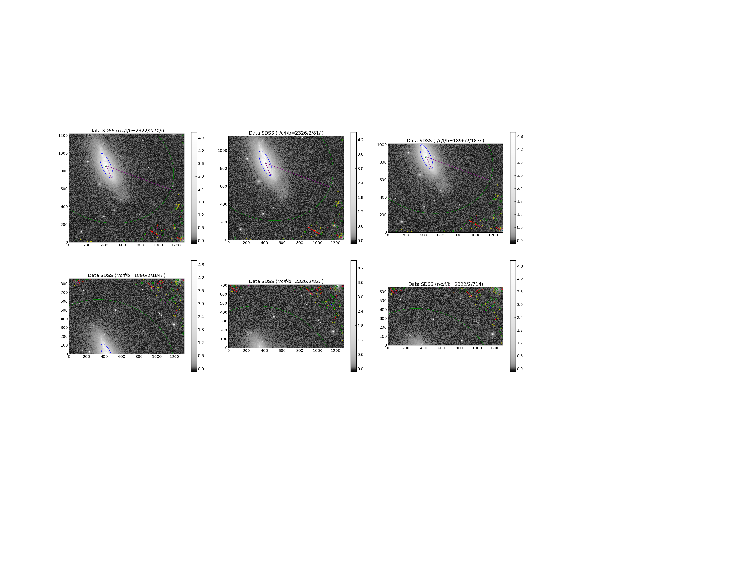
\includegraphics[trim = 1cm 3.2cm 3.8cm 2.15cm,clip=true,width=\textwidth] {data.pdf}
\caption{This shows the six different fields of data which are
 combined for the galaxy NGC 4605. The different fields represent
 different images taken by the Sloan telescope at different positions
 and different times.}
\label{fig:4605data}
\end{figure}

\begin{figure}
\centering
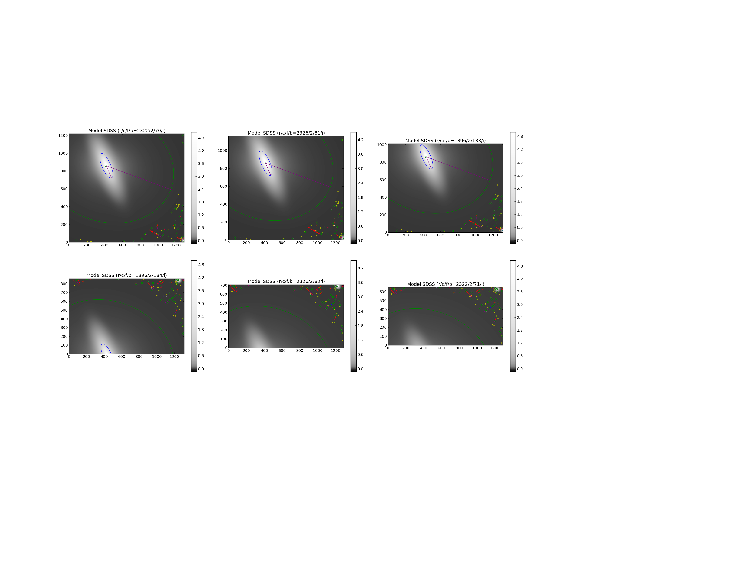
\includegraphics[trim = 1cm 3.2cm 3.8cm 2.15cm,clip=true,width=\textwidth] {model.pdf}
\caption{This is like fig \ref{fig:4605data} but shows the model we have built for the galaxy}
\label{fig:4605model}
\end{figure}

\begin{figure}
\centering
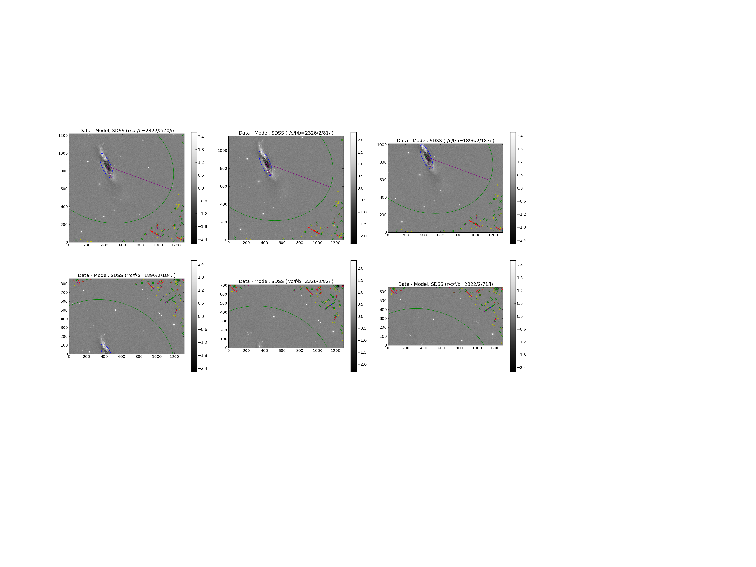
\includegraphics[trim = 1cm 3.2cm 3.8cm 2.15cm,clip=true,width=\textwidth] {diff.pdf}
\caption{This figure shows the difference between fig \ref{fig:4605data} and fig \ref{fig:4605model}}
\label{fig:4605diff}
\end{figure}

\begin{figure}
\centering
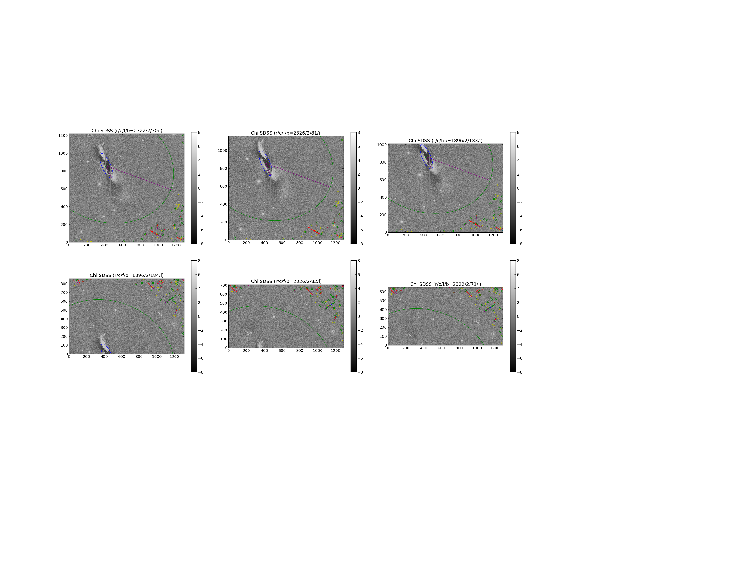
\includegraphics[trim = 1cm 3.2cm 3.8cm 2.15cm,clip=true,width=\textwidth] {chi.pdf}
\caption{This is the same as fig \ref{fig:4605diff} but shows the chi values, meaning that some pixels are masked out if they contain bad data.}
\label{fig:4605chi}
\end{figure}

\begin{figure}
\centering
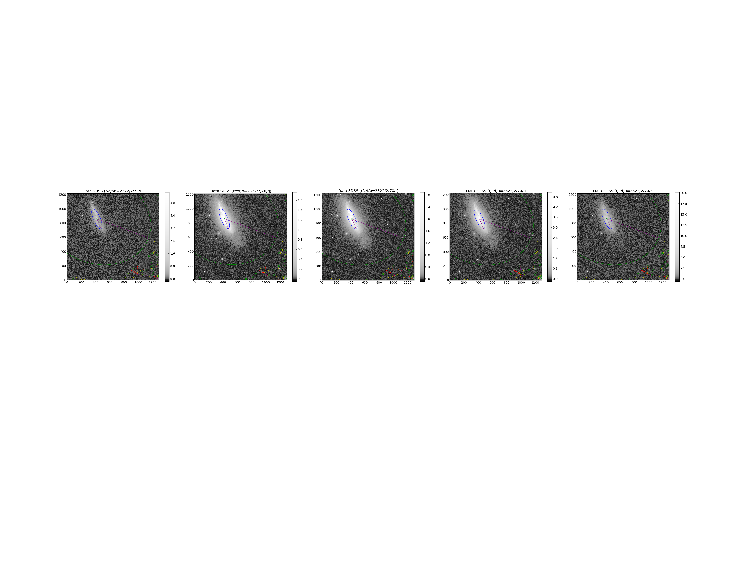
\includegraphics[trim = .9cm 4.5cm 0cm 2.9cm,clip=true,width=\textwidth] {goodsingle-colors-data.pdf}
\caption{This figure show the data for the five different bands for NGC 4605.}
\label{fig:colorsdata}
\end{figure}

\begin{figure}
\centering
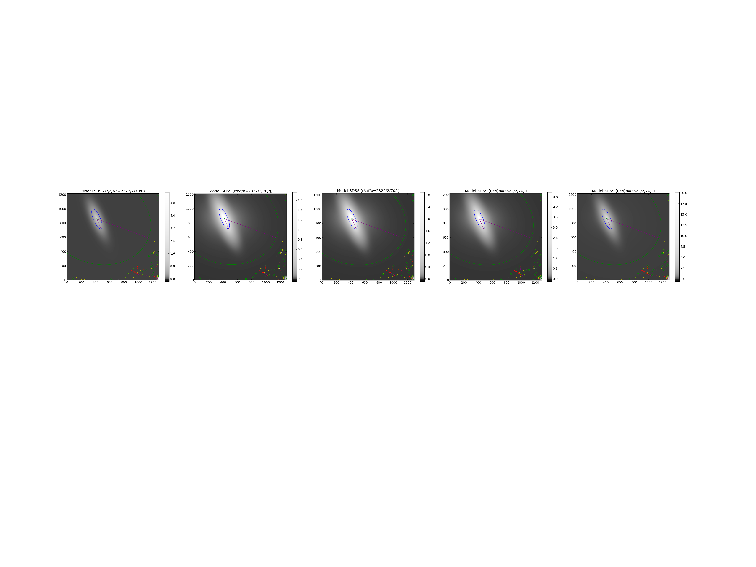
\includegraphics[trim = .9cm 4.5cm 0cm 2.9cm,clip=true,width=\textwidth] {goodsingle-colors-model.pdf}
\caption{This figure show the model for the five different bands for NGC 4605.}
\label{fig:colorsmodel}
\end{figure}

\begin{figure}
\centering
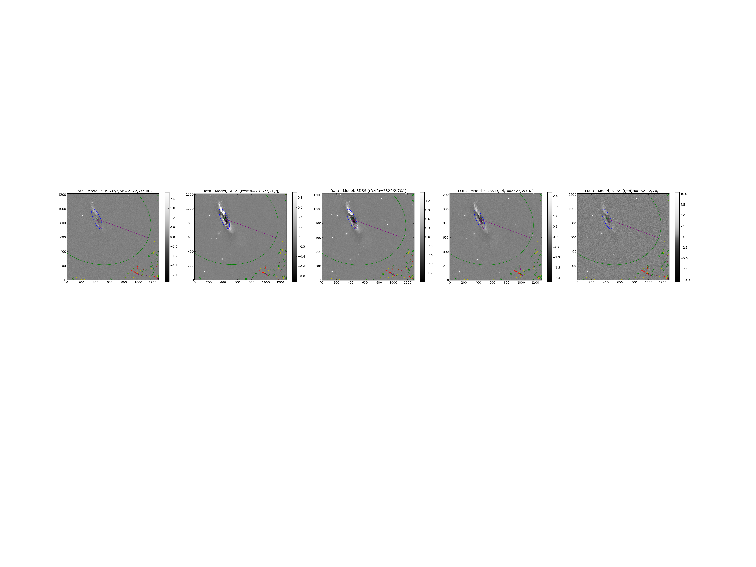
\includegraphics[trim = .9cm 4.5cm 0cm 2.9cm,clip=true,width=\textwidth] {goodsingle-colors-diff.pdf}
\caption{This figure show the diff for the five different bands for NGC 4605.}
\label{fig:colorsdiff}
\end{figure}

\begin{figure}
\centering
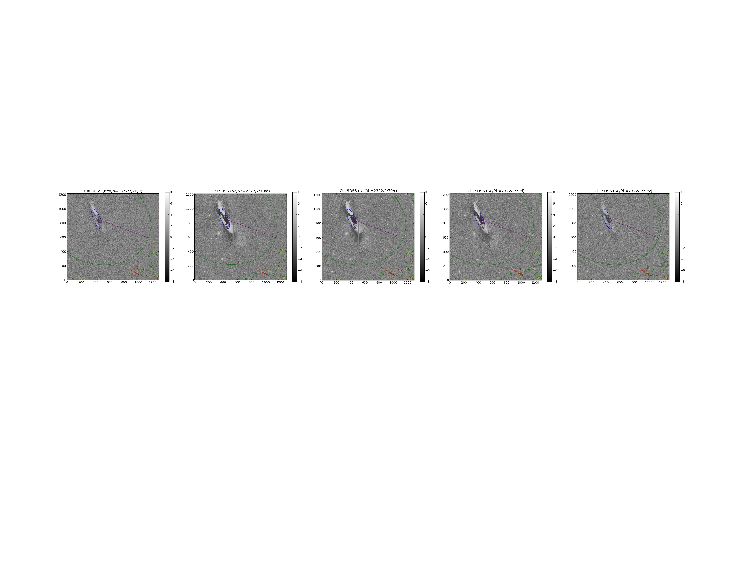
\includegraphics[trim = .9cm 4.5cm 0cm 2.9cm,clip=true,width=\textwidth] {goodsingle-colors-chi.pdf}
\caption{This figure show the chi for the five different bands for NGC 4605.}
\label{fig:colorschi}
\end{figure}

\begin{figure}
\centering
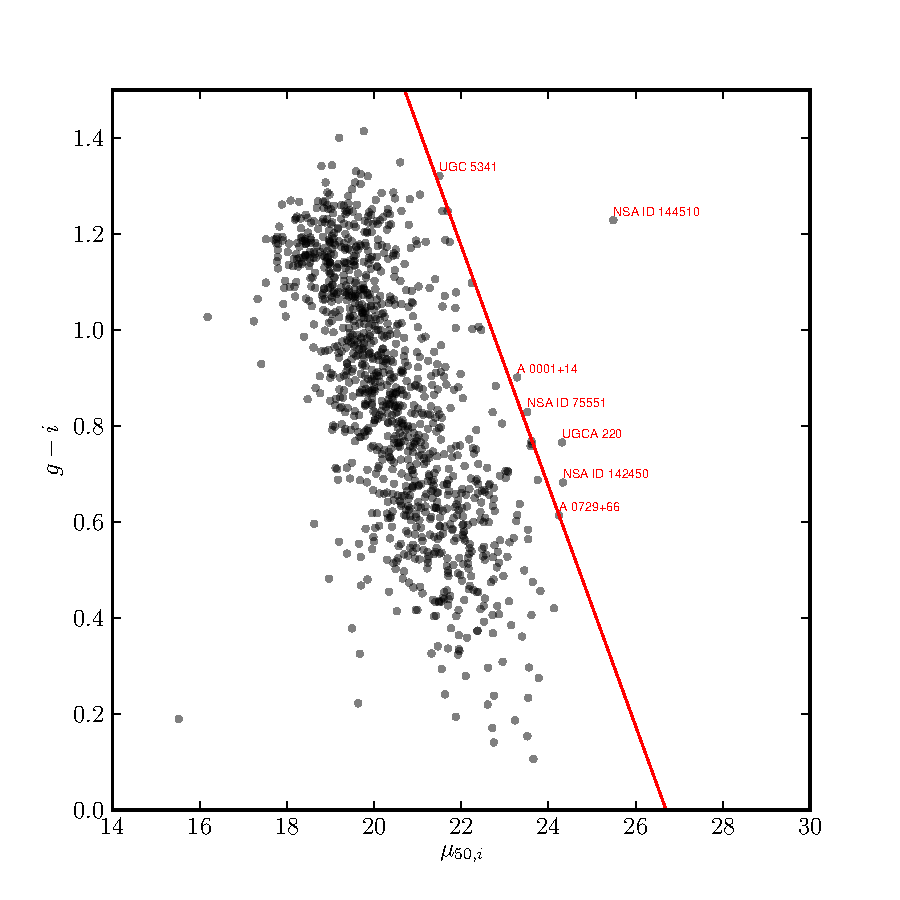
\includegraphics[trim= 0mm 0mm 0mm 10mm]{sb_color_outliers.pdf}
\caption{Surface brightness in the i-band using the half-light radius is plotted against the g-i color. Galaxies with truly low surfrace brightness that were consistent outliers on this plot as described in Section \ref{sec:handvetting} are labeled in red.}
\label{fig:outliers}
\end{figure}

\begin{figure}
\centering
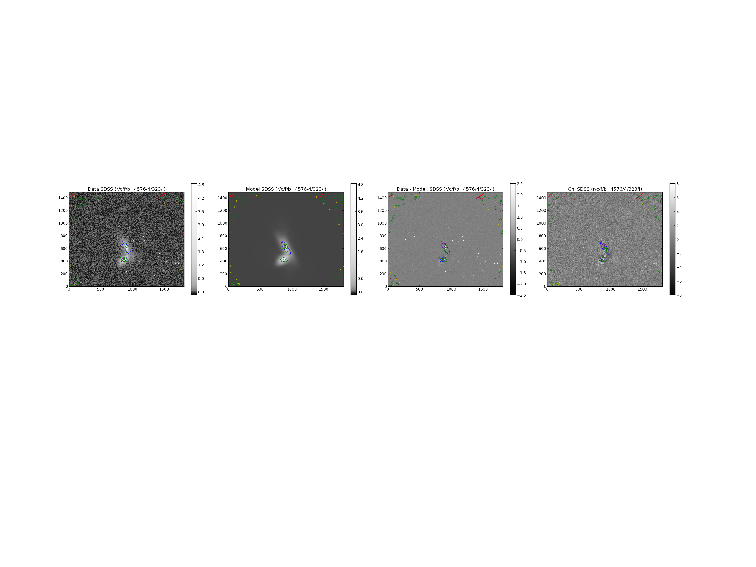
\includegraphics[trim = .9cm 4.5cm 1.15cm 2.9cm,clip=true,width=\textwidth] {gooddouble.pdf}
\caption{This figure show the fit for the galaxies NGC 3395 and NGC
 3396, which are fit simultaneously. From left to right, this shows
 the data, the model, the residues, and the chi values in just one of
 the fields.}
\label{fig:gooddouble}
\end{figure}

\begin{figure}
\centering
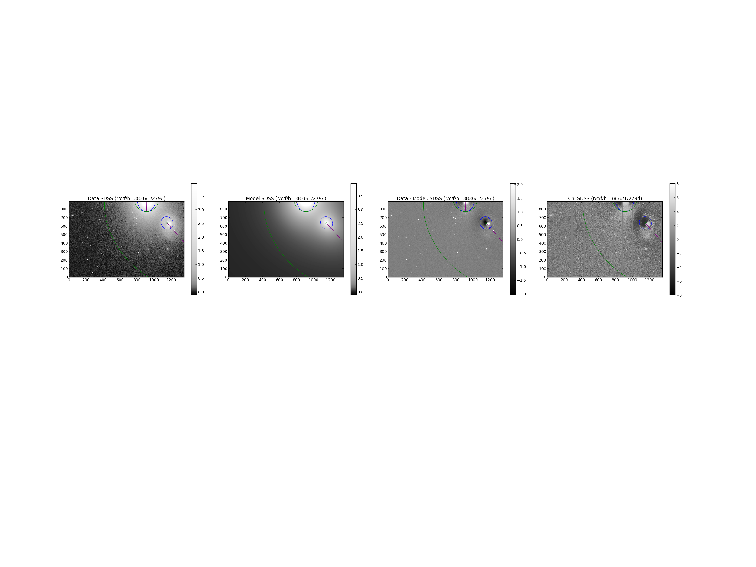
\includegraphics[trim = .9cm 4.5cm 1.15cm 2.9cm,clip=true,width=\textwidth] {baddouble.pdf}
\caption{This figure show the fit for the galaxies NGC 4647 and NGC
 4649. This example shows a failure of the attempt to fit two galaxies
 simultaneously. From left to right, this shows the data, the model,
 the residues, and the chi values in just one of the fields.}
\label{fig:baddouble}
\end{figure}

\begin{figure}
\centering
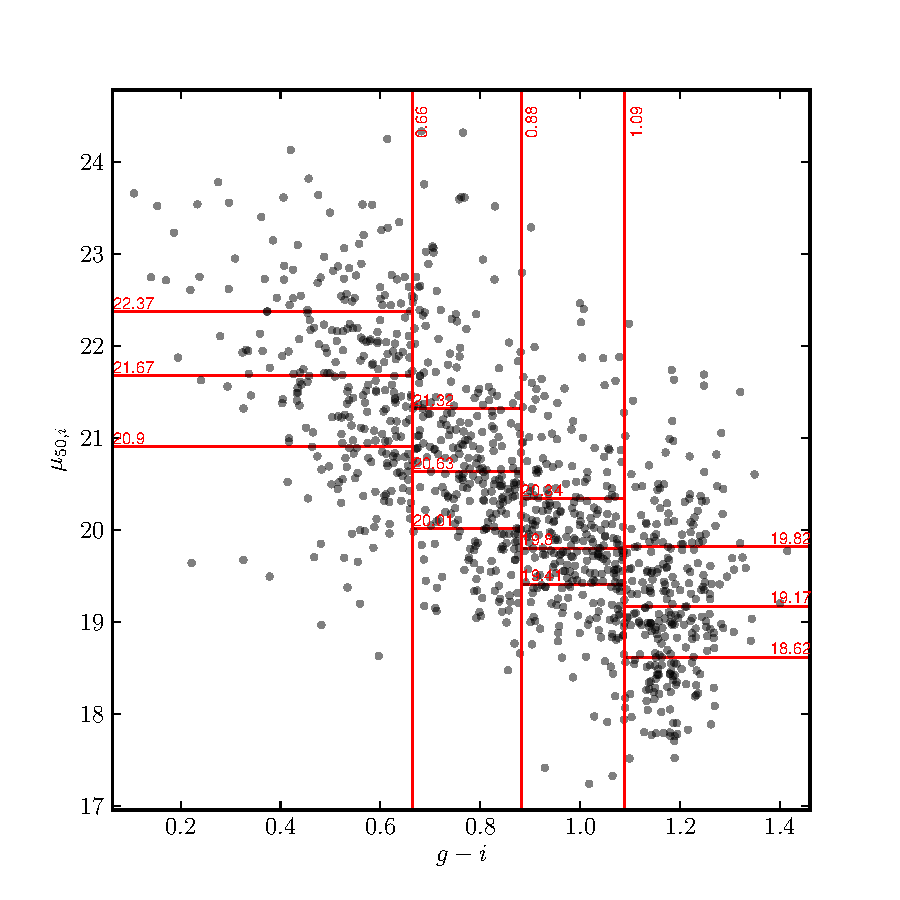
\includegraphics[trim=0mm 0mm 0mm 10mm]{quartiles.pdf}
\caption{Color versus surface brightness plotted for all galaxies in the SDSS LGA. The vertical lines have been plotted at the 25th, 50th and 75th percentiles in color. In each of those four quartiles, the 25th, 50th, and 75th percentile lines were drawn vertically.}
\label{fig:quartiles}
\end{figure}

\begin{figure}
\centering
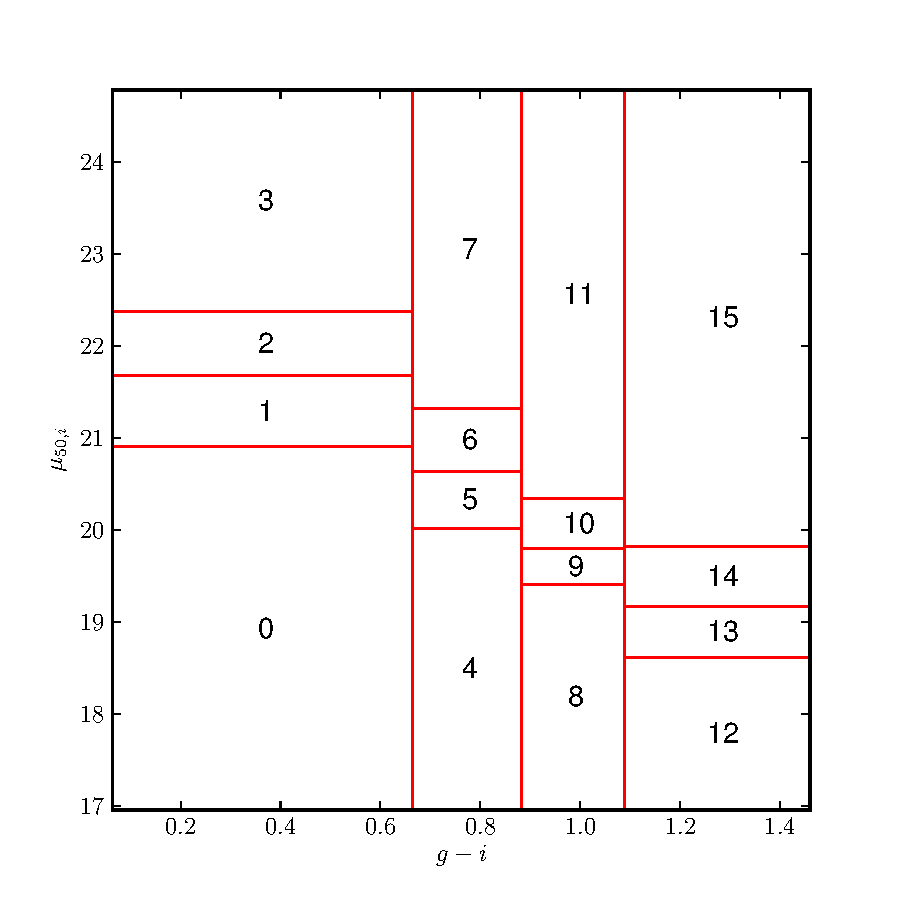
\includegraphics[trim =0mm 0mm 0mm 10mm]{quartile_diagram.pdf}
\caption{This diagram illustrates the labeling scheme used for quantiles described in \ref{sec:handvetting}. The lines represent the same quantities described in Figure \ref{fig:quartiles}.}
\label{fig:quartilediagram}
\end{figure}

\begin{figure}
\centering
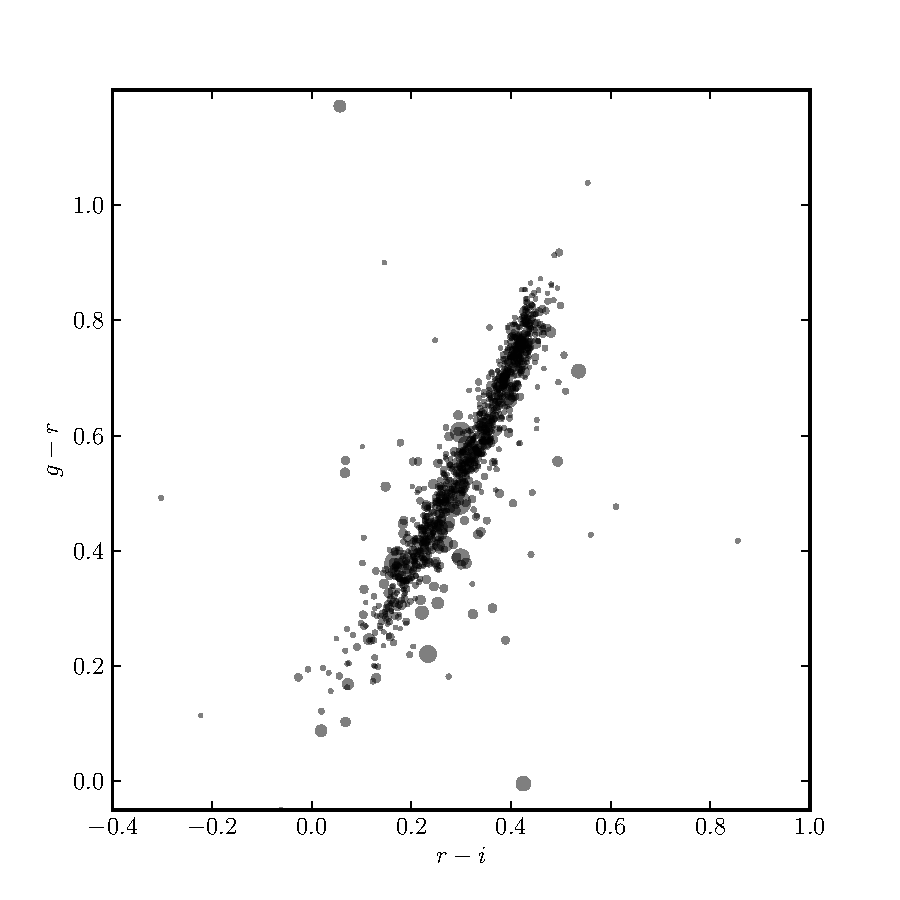
\includegraphics[trim= 0mm 0mm 0mm 10mm]{atlas_colors_size}
\caption{Colors for the data in the SDSS Large Galaxy Atlas. The g-r and r-i colors are shown with a very tight correlation for our 1100 galaxies. The colors here are already corrected with the SFD dust maps.They have been plotted with varying marker sizes proportional to the half-light radius in the i-band scaled down by a sixth of an arcminute.}
\label{fig:atlasconsistency}
\end{figure}

\begin{figure}
\centering
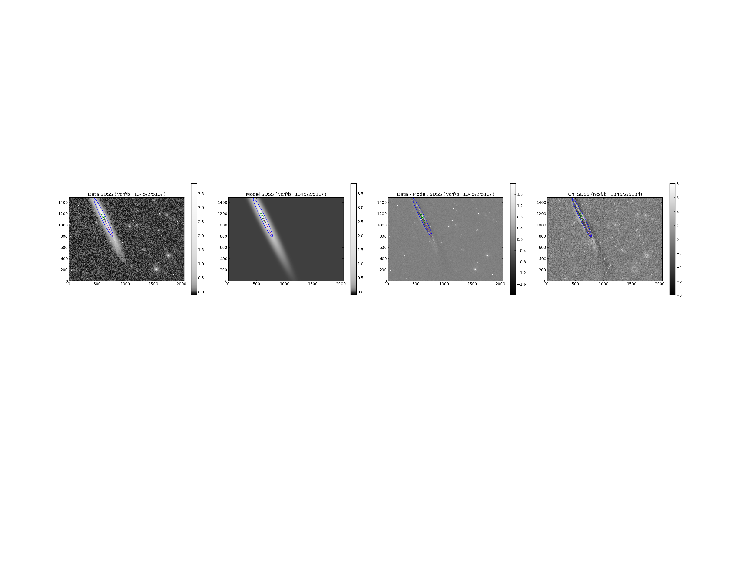
\includegraphics[trim = .9cm 4.5cm 1.15cm 2.9cm,clip=true,width=\textwidth] {edgeon.pdf}
\caption{This figure show the fit for the galaxy NGC 5907. This fit is
 bad because it fails on edge-on galaxies. From left to right, this
 shows the data, the model, the residues, and the chi values in just
 one of the fields.}
\label{fig:edgeon}
\end{figure}

\begin{figure}
\centering
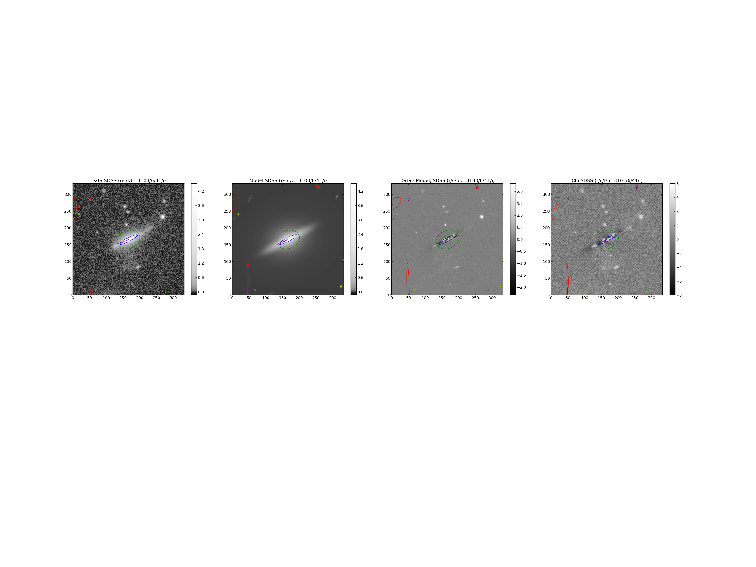
\includegraphics[trim = .9cm 4.5cm 1.15cm 2.9cm,clip=true,width=\textwidth]{badsingle.pdf}
\caption{This figure show the fit for the galaxy UGC 5613. This fit is
 bad because it fails to take into account that UGC 5613 is composed
 of a merger of two different galaxies, which causes our fit to
 fail. From left to right, this shows the data, the model, the
 residues, and the chi values in just one of the fields.}
\label{fig:badsingle}
\end{figure}

\clearpage

\begin{figure}
\centering
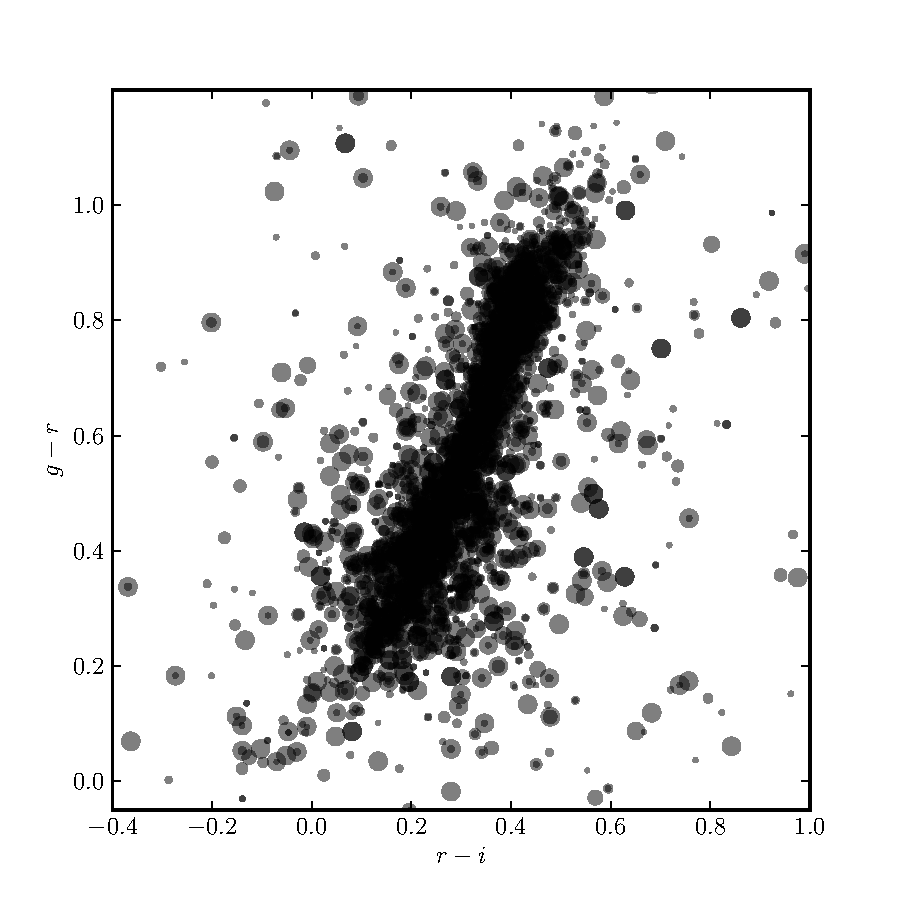
\includegraphics[trim=0mm 0mm 0mm 10mm, clip=true]{nsa_colors.pdf}
\caption{Colors for 2621 galaxies in the NSA are shown. Again, the g-r and the r-i colors are plotted, showing a wider distribution of color properties. The NSA galaxies given here are those which have a 50\% light radius of a 2D Sersic fit less than 158 arcseconds. A hard cut was also made to keep only galaxies with i and g band fluxes greater than zero to remove some inaccurate data. The NSA galaxies have also been extinction corrected using the SFD dust maps as given by \cite{blanton11}. The marker size is proportional to the sersic radius scaled down by a sixth of an arcminute.}
\label{fig:nsacolors}
\end{figure}

\begin{figure}
\centering
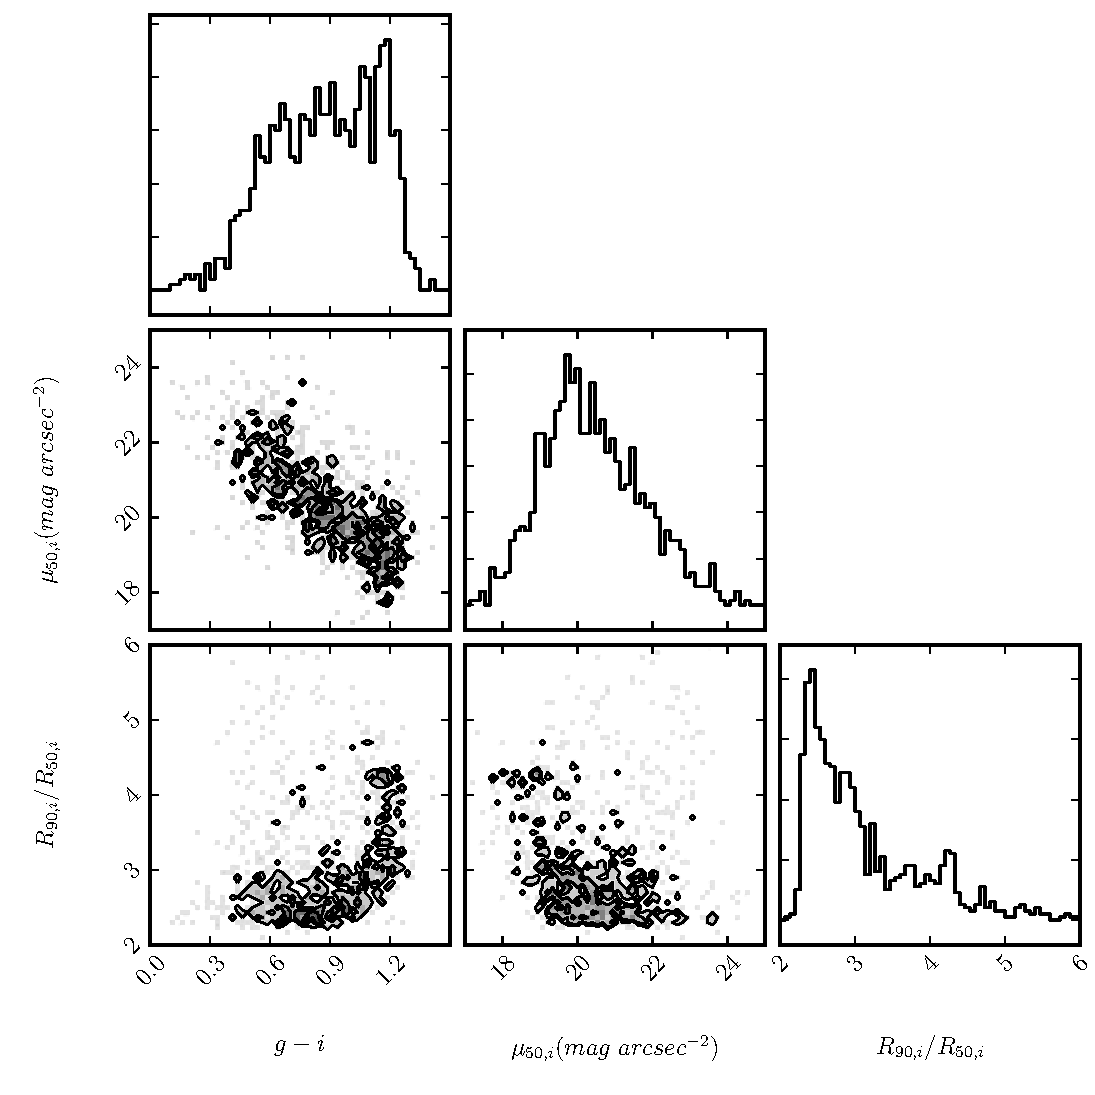
\includegraphics[trim=15mm 0mm 0mm 0mm]{color_sb_conc.pdf}
\caption{A triangle plot for the g-i color, i-band half-light surface brightness and i-band concentrations for the galaxies in the SDSS LGA.}
\label{fig:triangle}
\end{figure}

%% \begin{figure}
%% \centering
%% \includegraphics[trim=0mm 0mm 0mm 10mm, clip=true]{atlas_colors.pdf}
%% \caption{Colors for the data in the SDSS Atlas of Large Galaxies. The g-r and r-i colors are shown with a very tight correlation for our 1100 galaxies. The colors here are already corrected with the SFD dust maps.}
%% \label{fig:atlascolors}
%% \end{figure}

%% \begin{figure}
%% \centering
%% \includegraphics[trim= 15mm 0mm 0mm 0mm]{gi_mu_c.pdf}
%% \caption{A comparison of the g-i colors vs. surface brightness in the
%%  i-band vs. the ratio of half-light radius to 90\% light radius. The
%%  vertical lines provide the quartiles of the data set.}
%% \end{figure}

%% \begin{figure}
%% \centering
%% 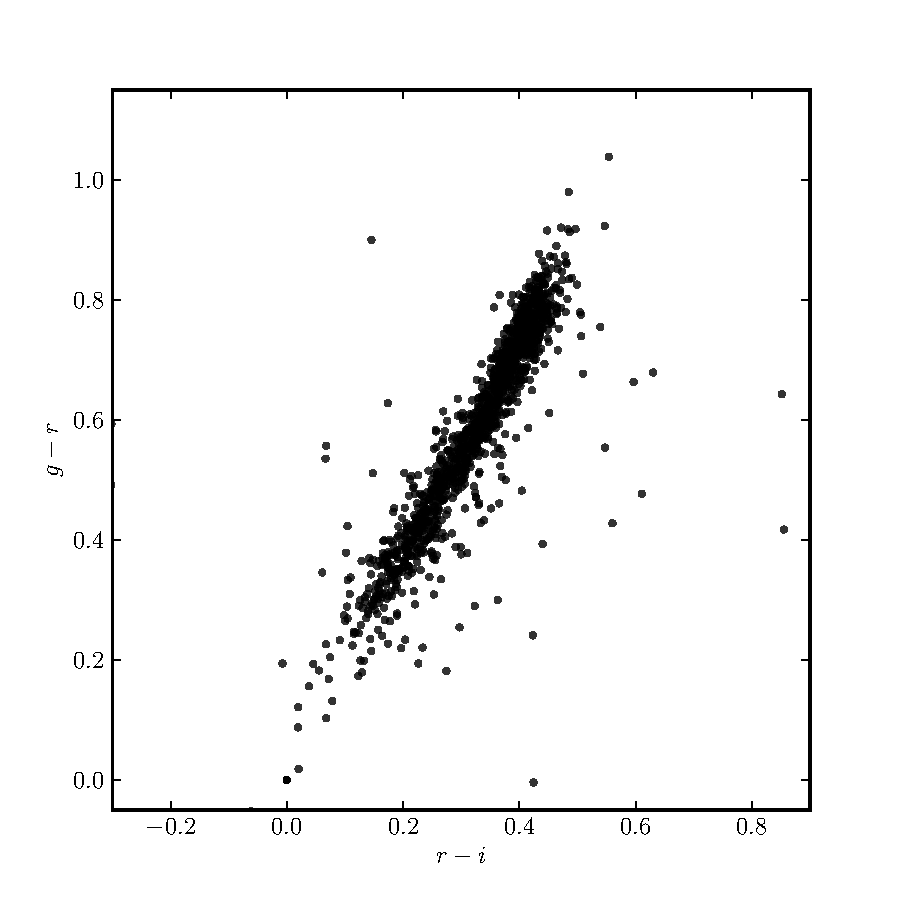
\includegraphics[trim = 15mm 0mm 0mm 0mm]{method_color_sloan.pdf}
%% \caption{A color-color plot of our Sloan Atlas data}
%% \end{figure}

%% \begin{figure}
%% \centering
%% 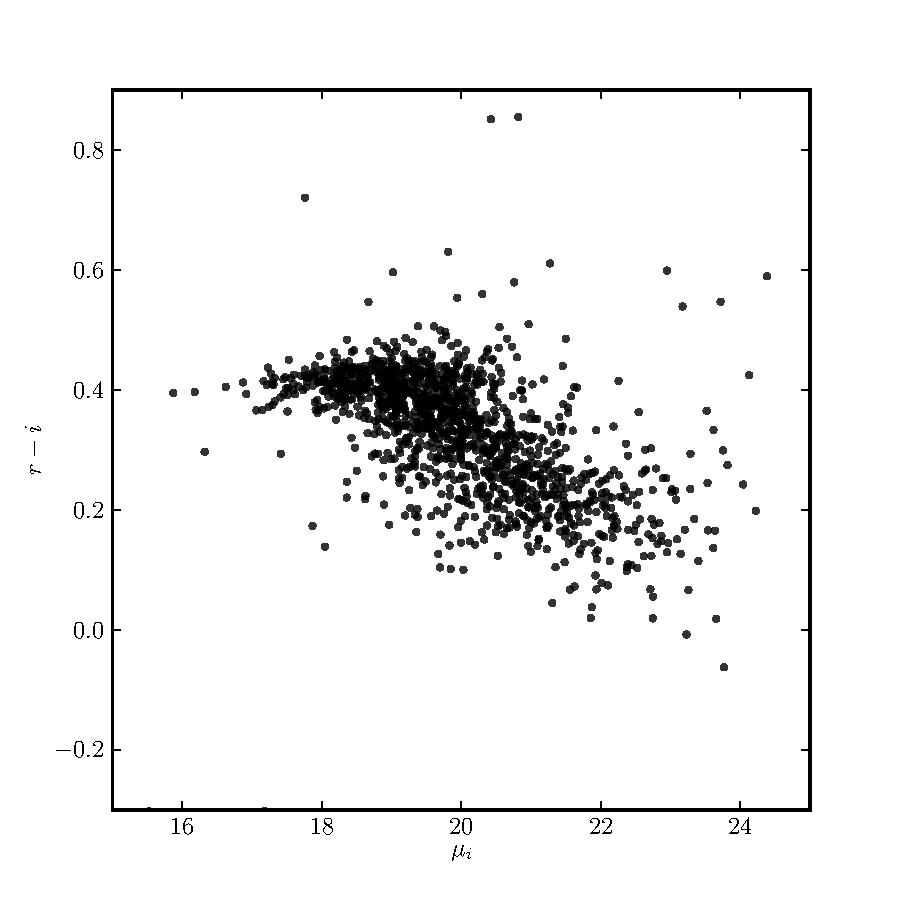
\includegraphics[trim = 15mm 0mm 0mm 0mm]{method_sb2_sloan.pdf}
%% \caption{Surface brightness in the i-band versus the r-i color for our Sloan Atlas data}
%% \end{figure}

%% \begin{figure}
%% \centering
%% 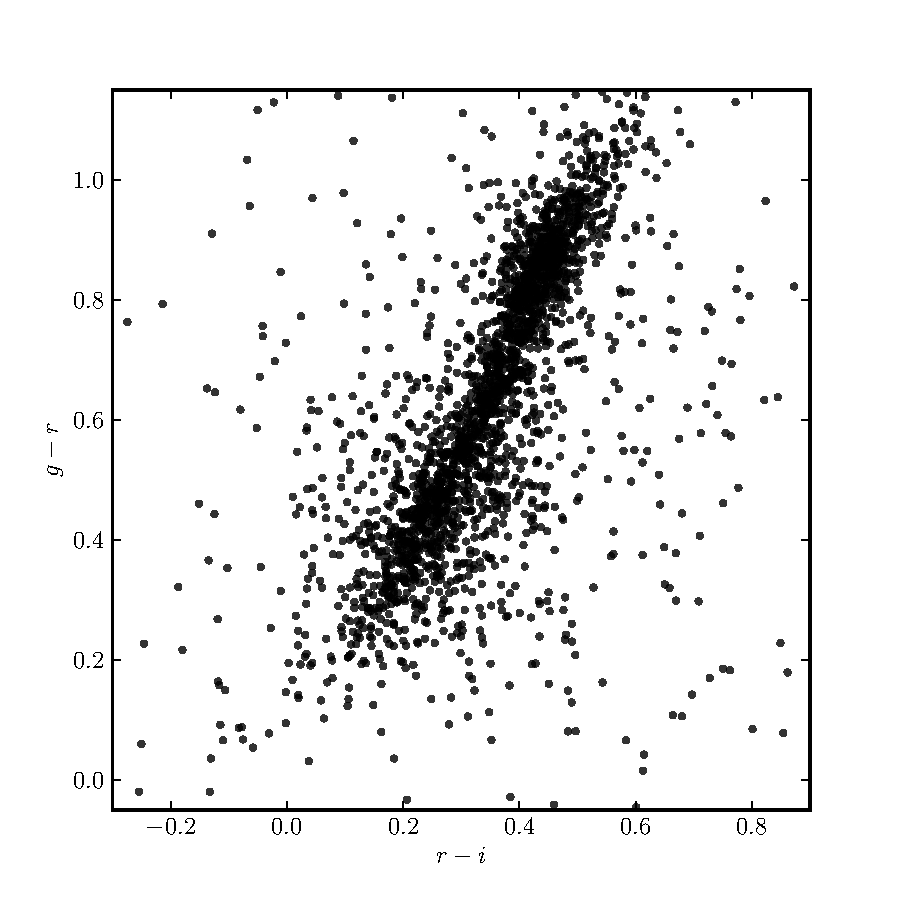
\includegraphics[trim = 15mm 0mm 0mm 0mm]{method_color_nsa.pdf}
%% \caption{A color-color plot of the NASA-Sloan Atlas data}
%% \end{figure}

%% \begin{figure}
%% \centering
%% 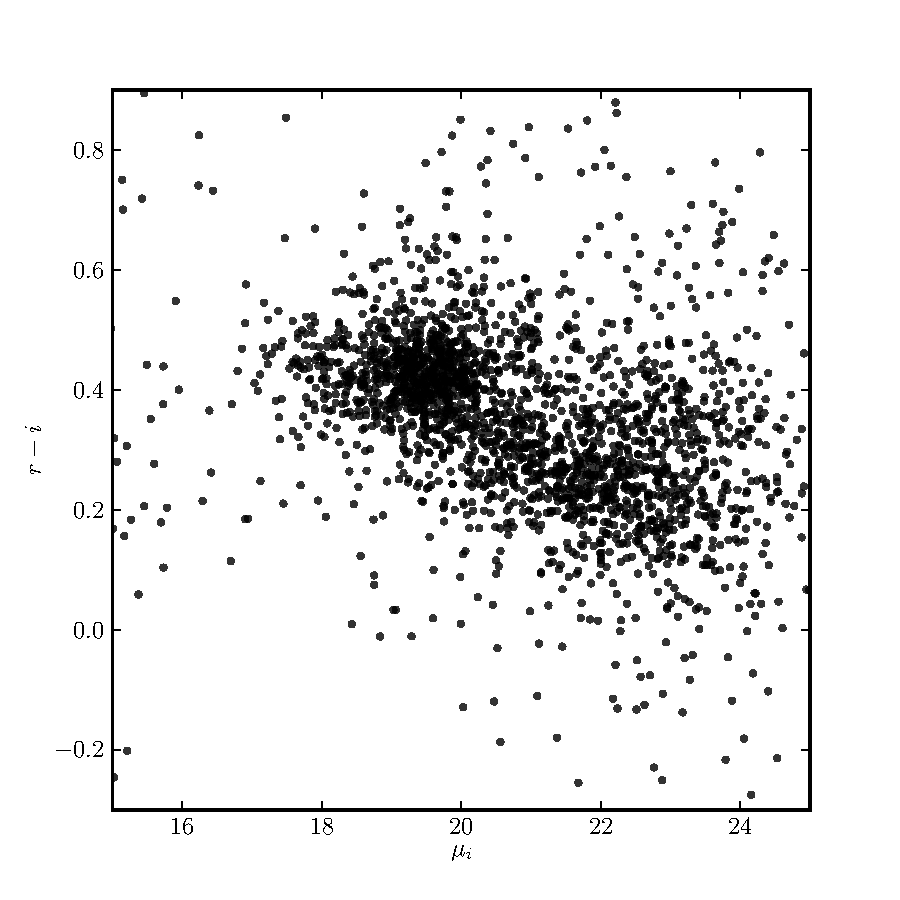
\includegraphics[trim = 15mm 0mm 0mm 0mm]{method_sb2_nsa.pdf}
%% \caption{Surface brightness in the i-band versus the r-i color for the NASA-Sloan Atlas data}
%% \end{figure}

\end{document}
